\section{Neuronová síť}
Neuronová síť je výpočetní model, který je inspirován fungováním lidského mozku.
Neuronová sít se skláda z tzv. umělých neuronů a váh.
Neurony jsou propojeny váhami mezi vrstvami.

Struktura neuronové sítě:
\begin{itemize}
    \item vstupní vrstva - zde se zadají vstupní data
    \item skryté vrstvy - tyto vrstvy transofrmují data a napomáhají řešit komplexní úlohy
    \item výstupní vrstva - vrací výsledky zpracování dat
\end{itemize}

Počty neuronů v každé vrstvě závisí na konkrétním využití a na problému, který má neuronová síť řešit.

Každý neuron představuje jednoduchý výpočetní prvek, který zpravová vstupy a generuje výstup.
Vstupy a výstupy jsou spojeny váhami, které ovlivňují hodnoty neuronů, ze kterých váha vede.
Dále má každý neuron svůj bias, který ovlivňuje jeho hodnotu.

\begin{figure}[h]
    \centering
    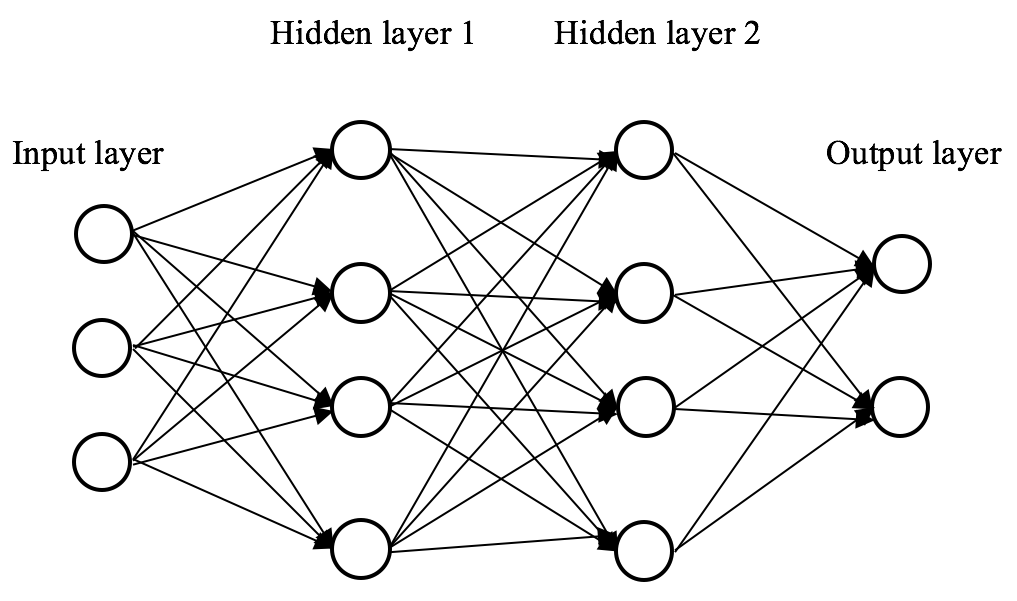
\includegraphics[width=0.75\textwidth]{images/network.png}
    \caption{Neuronová síť}\cite{sit}
\end{figure}

Existují různé typy neuronových sítí, které se liší tím, jak jsou neurony mezi vrstvami propojeny.
Různé typy propojení jsou vhodné pro různé typy úloh.
Mezi nejběžnější typy patří neuronové sítě typu perceptrony, vícevrstvé perceptory, konvulační neuronové sítě a rekurentní neuronové sítě.

Mezi hlavní výhody neuronových sítí patří schopnost učit se z dat a adaptovat se novým informacím.
Neuronové sítě dokáží řešit komplexní úlohy, které jsou extrémně náročné pro běžné algoritmy.
Tyto sítě jsou také vhodné pro práci s velými objemi dat.

\subsection{Fungování neuronových sítí}
Neuronová síť načte vstup a postupně se počítají hodnoty neuronů po vrstvách.
Až hodnoty projdou celou sítí nakonec, ve výstupní vrstvě je výsledek.

Hodnota konkrétního neuronu se spočítá z jeho vstupů. Každý neuron, až na vstupní vrstvu, má vstupní neurony.
Jeho hodnota se vypočíta ta, že se sečte hodnota všech jeho vstupních neuronů vynásobena spojujícími vahami každého neuronu.
Dále se přičte bias daného neuronu, který slouží jako práh aktivace. Nakonec se použije aktivační funkce.
Aktivačních funkcí je řada.
Mezi nejběžnější patří:
\[Sigmoid\quad \sigma(x) = \frac{1}{1 + e^{-x}}\]
\[ReLU\quad ReLU(x) = max(0, x)\]
\[Tanh\quad tanh(x) = \frac{e^{2x} - 1}{e^{2x} + 1}\]
Výběr ideální aktivační funkce opět zavisí na problému, který má síť řešit.
Tyto funkce v jednoduchosti transformují vstupy neuronu na jeho výstupy.
Aktivační funkce dodávají sítím jistou nelinearitu, která umožňuje sítím řešit i problémy, které nejsou linearní.

\begin{figure}[h]
    \centering
    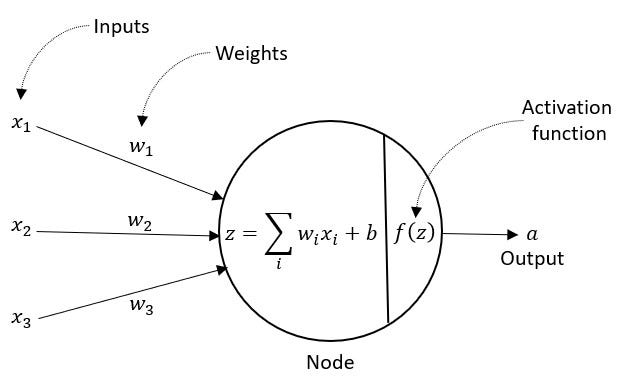
\includegraphics[width=0.75\textwidth]{images/neuron.jpg}
    \caption{Umělý neuron}\cite{umely_neuron}
\end{figure}

\newpage
